% Build from the repository root: sh docs/figures/build.sh
\documentclass[tikz,border=0pt]{standalone}
% Shared style for the cuPAMI README figures. Each figure \input's this file.
% Black and white only, serif type, as in a paper figure.
\usepackage[T1]{fontenc}
\usepackage{lmodern}
\usetikzlibrary{arrows.meta,shapes.geometric,backgrounds}
\newcommand{\head}[1]{{\large\bfseries #1}}
\newcommand{\sub}[1]{{\normalsize #1}}
\newcommand{\api}[1]{{\small\ttfamily #1}}
\tikzset{
 % Opaque white canvas so the figures stay readable in dark themes.
 canvas/.style={x=1cm,y=1cm,
  show background rectangle,inner frame sep=12pt,
  background rectangle/.style={fill=white}},
 box/.style={draw=black,line width=.8pt,fill=white,
  align=center,inner sep=7pt,minimum height=1.5cm,text width=3.8cm},
 core/.style={box,line width=1.6pt},
 ask/.style={diamond,aspect=2.1,draw=black,line width=.8pt,fill=white,
  align=center,inner sep=1pt,text width=2.9cm,
  minimum width=5cm,minimum height=2.4cm},
 region/.style={draw=black,line width=.5pt,dashed},
 flow/.style={-{Latex[length=2.6mm,width=1.9mm]},line width=.8pt,draw=black},
 note/.style={font=\normalsize,inner sep=3pt,align=center},
}

\begin{document}
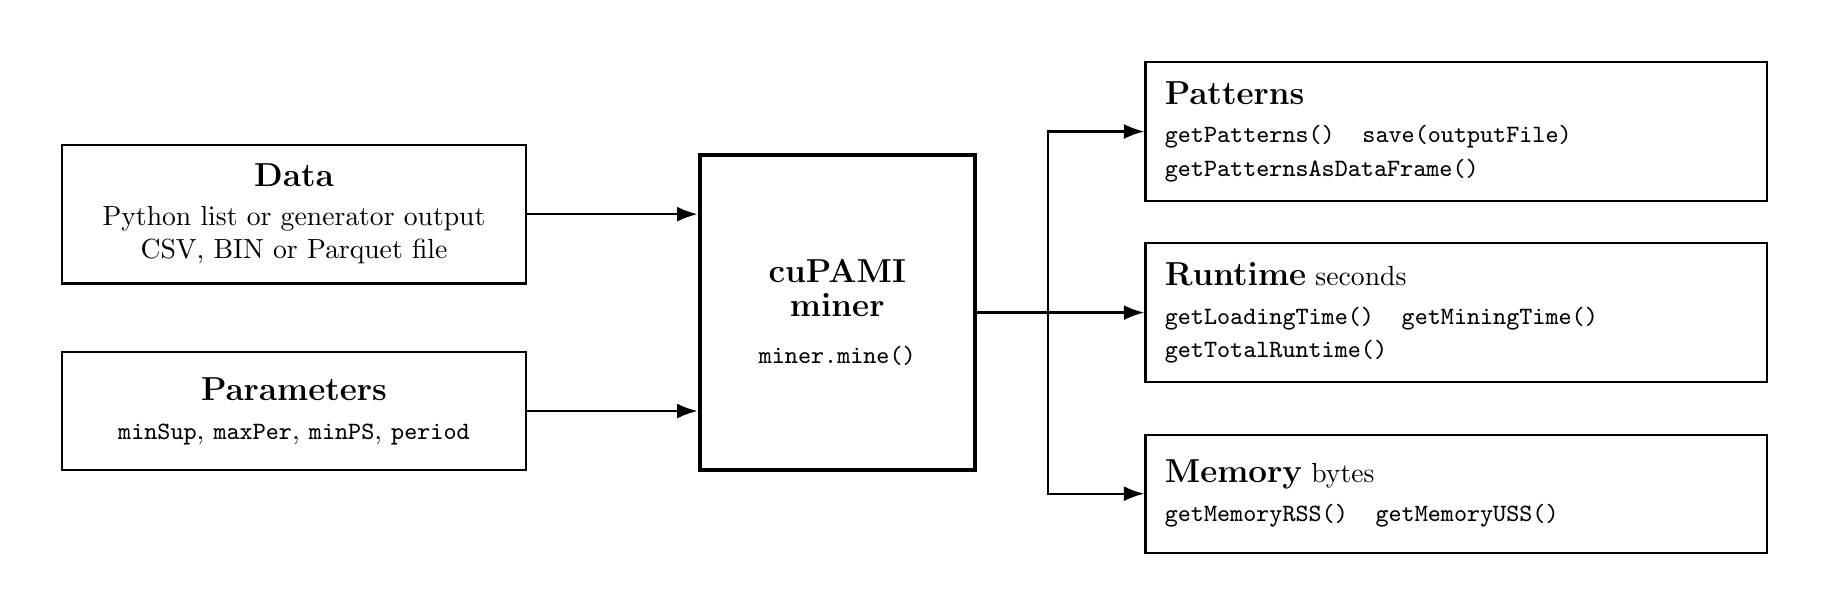
\begin{tikzpicture}[canvas,
 res/.style={box,align=left,text width=7.4cm,anchor=west}]
\node[box,text width=5.4cm] (data) at (0,1.25)
 {\head{Data}\\[2pt]\sub{Python list or generator output\\CSV, BIN or Parquet file}};
\node[box,text width=5.4cm] (params) at (0,-1.25)
 {\head{Parameters}\\[2pt]\api{minSup}, \api{maxPer}, \api{minPS}, \api{period}};
\node[core,text width=3cm,minimum height=4cm] (miner) at (6.9,0)
 {\head{cuPAMI miner}\\[5pt]\api{miner.mine()}};
\node[res] (patterns) at (10.8,2.3)
 {\head{Patterns}\\[2pt]\api{getPatterns()}\quad\api{save(outputFile)}\\
  \api{getPatternsAsDataFrame()}};
\node[res] (runtime) at (10.8,0)
 {\head{Runtime}\ \sub{seconds}\\[2pt]\api{getLoadingTime()}\quad\api{getMiningTime()}\\
  \api{getTotalRuntime()}};
\node[res] (memory) at (10.8,-2.3)
 {\head{Memory}\ \sub{bytes}\\[2pt]\api{getMemoryRSS()}\quad\api{getMemoryUSS()}};
\draw[flow] (data.east) -- (data.east -| miner.west);
\draw[flow] (params.east) -- (params.east -| miner.west);
\draw[flow] (miner.east) -- (runtime.west);
\draw[flow] (miner.east) -- ++(.9,0) |- (patterns.west);
\draw[flow] (miner.east) -- ++(.9,0) |- (memory.west);
\end{tikzpicture}
\end{document}
